\documentclass[hide notes,intlimits]{beamer}


\mode<presentation>
{
  \usetheme[footline]{UAFshade}
  \setbeamercovered{transparent}
}

% load packages
%\usepackage{media9}
%\usepackage{movie15}
\usepackage{multimedia}
\usepackage[english]{babel}
\usepackage[latin1]{inputenc}
\usepackage[T1]{fontenc}
\usepackage{lmodern}
\usepackage[multidot]{grffile}

\usepackage{tikz}
\usetikzlibrary{shapes,arrows,shadows, calc}


\definecolor{dark red}{HTML}{E41A1C}
\definecolor{dark green}{HTML}{4DAF4A}
\definecolor{dark violet}{HTML}{984EA3}
\definecolor{dark blue}{HTML}{084594}
\definecolor{dark orange}{HTML}{FF7F00}
\definecolor{light blue}{HTML}{377EB8}
\definecolor{light red}{HTML}{FB9A99}
\definecolor{light violet}{HTML}{CAB2D6}

\definecolor{uaf red}{HTML}{E41A1C}
\definecolor{uaf blue}{HTML}{377EB8}
\definecolor{uaf green}{HTML}{4DAF4A}
\definecolor{uaf violet}{HTML}{984EA3}
\definecolor{uaf orange}{HTML}{FF7F00}
\setbeamercolor{boxed}{fg=black,bg=uaf yellow}

\graphicspath{{figures/}}

\setbeamerfont{caption}{size=\scriptsize}

% code adapted from http://tex.stackexchange.com/a/11483/3954

% some parameters for customization
\def\shadowshift{3pt,-3pt}
\def\shadowradius{6pt}

\colorlet{innercolor}{black!60}
\colorlet{outercolor}{gray!05}

% this draws a shadow under a rectangle node
\newcommand\drawshadow[1]{
    \begin{pgfonlayer}{shadow}
        \shade[outercolor,inner color=innercolor,outer color=outercolor] ($(#1.south west)+(\shadowshift)+(\shadowradius/2,\shadowradius/2)$) circle (\shadowradius);
        \shade[outercolor,inner color=innercolor,outer color=outercolor] ($(#1.north west)+(\shadowshift)+(\shadowradius/2,-\shadowradius/2)$) circle (\shadowradius);
        \shade[outercolor,inner color=innercolor,outer color=outercolor] ($(#1.south east)+(\shadowshift)+(-\shadowradius/2,\shadowradius/2)$) circle (\shadowradius);
        \shade[outercolor,inner color=innercolor,outer color=outercolor] ($(#1.north east)+(\shadowshift)+(-\shadowradius/2,-\shadowradius/2)$) circle (\shadowradius);
        \shade[top color=innercolor,bottom color=outercolor] ($(#1.south west)+(\shadowshift)+(\shadowradius/2,-\shadowradius/2)$) rectangle ($(#1.south east)+(\shadowshift)+(-\shadowradius/2,\shadowradius/2)$);
        \shade[left color=innercolor,right color=outercolor] ($(#1.south east)+(\shadowshift)+(-\shadowradius/2,\shadowradius/2)$) rectangle ($(#1.north east)+(\shadowshift)+(\shadowradius/2,-\shadowradius/2)$);
        \shade[bottom color=innercolor,top color=outercolor] ($(#1.north west)+(\shadowshift)+(\shadowradius/2,-\shadowradius/2)$) rectangle ($(#1.north east)+(\shadowshift)+(-\shadowradius/2,\shadowradius/2)$);
        \shade[outercolor,right color=innercolor,left color=outercolor] ($(#1.south west)+(\shadowshift)+(-\shadowradius/2,\shadowradius/2)$) rectangle ($(#1.north west)+(\shadowshift)+(\shadowradius/2,-\shadowradius/2)$);
        \filldraw ($(#1.south west)+(\shadowshift)+(\shadowradius/2,\shadowradius/2)$) rectangle ($(#1.north east)+(\shadowshift)-(\shadowradius/2,\shadowradius/2)$);
    \end{pgfonlayer}
}

% create a shadow layer, so that we don't need to worry about overdrawing other things
\pgfdeclarelayer{shadow} 
\pgfsetlayers{shadow,main}

\newsavebox\mybox
\newlength\mylen

\newcommand\shadowimage[2][]{%
\setbox0=\hbox{\includegraphics[#1]{#2}}
\setlength\mylen{\wd0}
\ifnum\mylen<\ht0
\setlength\mylen{\ht0}
\fi
\divide \mylen by 120
\def\shadowshift{\mylen,-\mylen}
\def\shadowradius{\the\dimexpr\mylen+\mylen+\mylen\relax}
\begin{tikzpicture}
\node[anchor=south west,inner sep=0] (image) at (0,0) {\includegraphics[#1]{#2}};
\drawshadow{image}
\end{tikzpicture}}

\newcommand\shadowimagec[3][]{%
\setbox0=\hbox{\includegraphics<#1>[#2]{#3}}
\setlength\mylen{\wd0}
\ifnum\mylen<\ht0
\setlength\mylen{\ht0}
\fi
\divide \mylen by 120
\def\shadowshift{\mylen,-\mylen}
\def\shadowradius{\the\dimexpr\mylen+\mylen+\mylen\relax}
\begin{tikzpicture}
\node[anchor=south west,inner sep=0] (image) at (0,0) {\includegraphics<#1>[#2]{#3}};
\drawshadow{image}
\end{tikzpicture}}


\newenvironment{transbox}[1][]{%
\begin{tikzpicture}
\node[drop shadow,rounded corners,text width=\textwidth,fill=white, fill opacity=#1,text opacity=1] \bgroup
}{
\egroup;\end{tikzpicture}} 

\newenvironment{transbox-tight}{%
\begin{tikzpicture}
\node[drop shadow,rounded corners,fill=uaf yellow, fill opacity=0.75,text opacity=1] \bgroup
}{
\egroup;\end{tikzpicture}} 


% title page
\title[] % (optional, use only with long paper titles)
{Pulling the plug}

\subtitle{When Greenland's outlet glaciers speed up}


\author[Aschwanden] % (optional, use only with lots of authors)
{Andy Aschwanden}
% - Give the names in the same order as the appear in the paper.
% - Use the \inst{?} command only if the authors have different
%   affiliation.

\institute[Geophysical Institute] % (optional, but mostly needed)
{Geophysical Institute}
% - Use the \inst command only if there are several affiliations.
% - Keep it simple, no one is interested in your street address.

\titlegraphic{\vskip-0.5cm\includegraphics[width=\textwidth]{gris-nw-speed-exp-600m}}

\date{}

\begin{document}

% define what is shown at the beginning of each section
\AtBeginSection[]
{
  \begin{frame}<handout:0>
    \frametitle{Outline}
   \tableofcontents[currentsection,subsectionstyle=hide/hide/hide]
  \end{frame}
}

% define what is shown at the beginning of each subsection
\AtBeginSubsection[]
{
 \begin{frame}<beamer>
  \frametitle{Outline}
   \tableofcontents[currentsection,currentsubsection]
 \end{frame}
}



\setbeamertemplate{background canvas}
  {
     \tikz{\node[inner sep=0pt,opacity=1.0] {\includegraphics[width=\paperwidth]{uaf_beamer_shade_bg}};}
} 


% insert titlepage
\begin{frame}
  \titlepage
\end{frame}


\setbeamertemplate{background canvas}
  {
     \tikz{\node[inner sep=0pt,opacity=1] {\includegraphics[height=\paperheight,width=\paperwidth]{taku-heli}};}
} 

\begin{frame}[plain]
\end{frame}



\setbeamertemplate{background canvas}
  {
     \tikz{\node[inner sep=0pt,opacity=1] {\includegraphics[height=\paperheight,width=\paperwidth]{nasa-mapping-greenland-ice-sheet}};}
} 

\begin{frame}[plain]
\end{frame}

\setbeamertemplate{background canvas}
  {
     \tikz{\node[inner sep=0pt,opacity=.5] {\includegraphics[height=\paperheight,width=\paperwidth]{nasa-mapping-greenland-ice-sheet}};}
} 

\begin{frame}[plain]
    \begin{itemize}
    \item extent of $1200\,\text{km}\,\times 2400\,\text{km}$ \dots it's a ``dwarf continent''
    \item has ice equivalent to 7 m of sea-level rise
    \item over past 2 decades: losing mass at an accelerating rate
    \end{itemize}
\end{frame}


\setbeamertemplate{background canvas}
{
%
} 

\begin{frame}[plain]
    \begin{figure}
      \movie[showcontrols=true,loop,width=12cm]{\includegraphics[width=12cm]{grace_greenland_2004_2012_still_print}}{grace_greenland_2004_2013_1080p.mov}
  \end{figure}
\end{frame}


\setbeamertemplate{background canvas}
  {
     \tikz{\node[inner sep=0pt,opacity=.5] {\includegraphics[height=\paperheight,width=\paperwidth]{nasa-mapping-greenland-ice-sheet}};}
} 

\begin{frame}[plain]
  \textbf{The increase in mass loss is roughly equally split between changes in}
    \begin{columns}[c]
      \begin{column}{.28\linewidth}
        \begin{figure}
          \includegraphics[width=\linewidth]{gris-melt-ponds}
        \end{figure}
      \end{column}
      \begin{column}{.67\linewidth}
        \textbf{surface mass balance}
      \end{column}
    \end{columns}
    \begin{columns}[c]
      \begin{column}{.28\linewidth}
        \begin{figure}
          \includegraphics<1>[width=\linewidth]{storeglacier}
        \end{figure}
      \end{column}
      \begin{column}{.67\linewidth}
        \textbf{ice discharge}
      \end{column}
    \end{columns}

\end{frame}


\setbeamertemplate{background canvas}
{
%
} 


\begin{frame}{How does an ice sheet lose mass?}
  \begin{figure}
    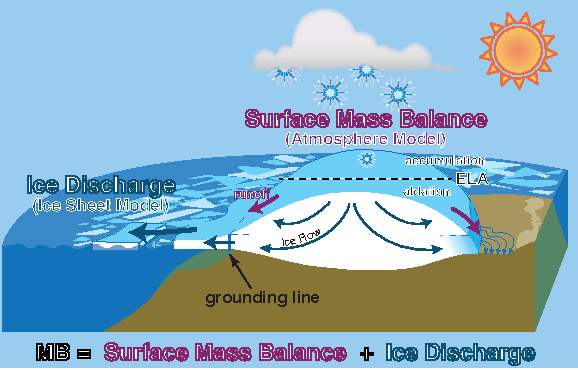
\includegraphics[width=.96\textwidth]{ice-sheet-cartoon}
  \end{figure}
  \note[item]{explain surface melt, ice discharge/calving, and basal melt}
  \note[item]{before the mid-90s mass loss was dominated by surface mass balance (80-90\%)}
  \note[item]{contribution of ice discharge was modest (10--20\%)}
  \note[item]{explaining in more detail in the next slide}
\end{frame}



\setbeamertemplate{background canvas}
  {
     \tikz{\node[inner sep=0pt,opacity=.75] {\includegraphics[height=\paperheight,width=\paperwidth]{outlet-glacier-collage-01}};}
}

\begin{frame}[plain]
    \begin{itemize}
    \item ice discharge to the ocean mostly through 200+ ``outlet glaciers''
    \item outlet glaciers are flowing fast ($>$200\,m/yr), are controlled by bedrock geometry, and terminate in narrow fjords ($<$10\,km wide)
    \end{itemize}
\end{frame}
 

\setbeamertemplate{background canvas}
{
%
} 


\begin{frame}{Jakobshavn Isbr{\ae}, west Greenland}
 \begin{figure}
    \includegraphics[height=.8\textheight]{MODISGreenlandJakobshavn} \\
    \scriptsize{based on MODIS data from M. Fahnestock}
  \end{figure}
  \note[item]{Jakobshavn serves as example to show observed changes}
  \note[item]{Greenland's biggest and fastest flowing outlet glacier}
  \note[item]{drains about 7\% of the entire ice sheet}
\end{frame}

\begin{frame}{Jakobshavn Isbr{\ae}, west Greenland}
 \begin{figure}
    \includegraphics[width=\textwidth]{Jakobshavn_groundline_retreat} \\
  \end{figure}
  \note[item]{Echelmeyer and Harrison investigated Jakobshavn in the mid-80s}
  \note[item]{found high flow speeds but the lack of seasonal variations}
  \note[item]{relatively steady behavior}
  \note[item]{seasonal variations in flow speed in 1995}
  \note[item]{and in 1997, the glacier suddenly switched from slow thickening to rapid thinning}
  \note[item]{caused by an increase in subsurface ocean temperature from 1.7degC in 1995 to 3.3degC in 1998, leading to increased melting}
  \note[item]{In summer 1998 the first major increase in surface velocity was seen}
  \note[item]{first departure from the normal pattern of frontal positions 1998}
  \note[item]{retreat of the ice front started around 2002}
\end{frame}

\begin{frame}{Jakobshavn Isbr{\ae}, west Greenland}
 \begin{figure}
    \includegraphics<1>[width=\textwidth]{jib-front-1990}
    \includegraphics<2>[width=\textwidth]{jib-front-2005}
    \includegraphics<3>[width=\textwidth]{jib-front-1990-2005-change}
    \includegraphics<4>[width=\textwidth]{jib-front-1990-2005-plug}
  \end{figure}
\end{frame}


\begin{frame}{Speed-up of Jakobshavn Isbr{\ae} 1992-2000}
  \begin{itemize}
    \item almost doubled its flow speed between the 1992 and 2000
  \end{itemize}
  \begin{figure}
    \includegraphics[width=\textwidth]{Joughin2004Fig2} \\
    \footnotesize{Joughin et al. (2004)}
  \end{figure}
  \note[item]{illustration of the speed up}
\end{frame}


\begin{frame}{}
  ice sheet models are needed to understand these changes
\end{frame}


\begin{frame}{What is an ice sheet model?}
  \begin{figure}
    \includegraphics[width=8cm]{grn_system_eqns}
  \end{figure}
  \begin{columns}[c]
    \begin{column}{.40\linewidth}
      \begin{itemize}
      \item ice dynamics
      \item thermodynamics
      \item surface processes
      \end{itemize}
    \end{column}
    \begin{column}{.55\linewidth}
      \begin{itemize}
      \item boundary conditions
      \item hydrology
      \item ice-ocean interaction (e.g. calving)
      \end{itemize}
    \end{column}
  \end{columns}
  \note[item]{An ice sheet model solves numerical approximations to the balance equations of mass, momentum}
  \note[item]{Ice flow is governed by Stokes equations with a power-law rheology}
  \note[item]{Because the viscosity of ice strongly depends on the thermal state, we also need to solve an energy balance equation}
  \note[item]{This makes the problem thermomechanically-coupled.}
  \note[item]{some processes such as hydrology are currently only parametrized}
\end{frame}


\begin{frame}{Why ice sheet modeling is easy}
  \begin{columns}[c]
    \begin{column}{.28\linewidth}
      \begin{figure}
        \includegraphics<1>[width=\linewidth]{ggstokes}
        \\ \scriptsize{G.~G.~Stokes}
      \end{figure}
    \end{column}
    \begin{column}{.67\linewidth}
      \begin{itemize}
      \item composed of a single, largely homogenous material
      \item flow governed by the Stokes equations known since the mid-19th century
      \item flows slowly: we can ignore turbulence, Coriolis and other inertial effects
      \end{itemize}
    \end{column}
  \end{columns}
\end{frame}


\begin{frame}{Why ice sheet modeling is so hard}
    \begin{columns}[c]
      \begin{column}{.28\linewidth}
        \begin{figure}
          \includegraphics<1>[width=\linewidth]{storeglacier}
        \end{figure}
      \end{column}
      \begin{column}{.67\linewidth}
        \begin{block}{Boundary conditions}
        \begin{itemize}
        \item seaward margin boundary condition
        \item basal boundary condition
        \end{itemize}
      \end{block}
      \end{column}
    \end{columns}
    \begin{columns}[c]
      \begin{column}{.28\linewidth}
        \begin{figure}
          \includegraphics<1>[width=\linewidth]{canale_grande_V05}
        \end{figure}
      \end{column}
      \begin{column}{.67\linewidth}
        \begin{block}{Initial conditions}
        \begin{itemize}
        \item ice thickness / subglacial topography is a first order constraint on ice flow
        \end{itemize}
      \end{block}
      \end{column}
    \end{columns}
    \begin{columns}[c]
      \begin{column}{.3\linewidth}
        \begin{figure}
          \includegraphics<1>[width=\linewidth]{bw_front_sm}
        \end{figure}
      \end{column}
      \begin{column}{.67\linewidth}
        \begin{block}{Computational costs}
        \begin{itemize}
        \item solving the Stokes equations is computationally very expensive
        \end{itemize}
      \end{block}
      \end{column}
    \end{columns}
\end{frame}


\begin{frame}{Challenge: basal boundary condition}
  \begin{columns}[c]
    \begin{column}{.50\linewidth}
      \begin{figure}
        \scriptsize{basal resistance} \\
        \includegraphics[width=\textwidth]{tauc}
      \end{figure}
    \end{column}
    \begin{column}{.5\linewidth}
      \begin{itemize}
      \item stresses vary by orders of magnitude
      \item transience and complexity of basal water flow
      \item despite more than 5 decades of research, we only have crude parametrizations
      \end{itemize}
    \end{column}
  \end{columns}
  \note[item]{First, stresses at the base vary by several orders of magnitude}
  \note[item]{depend on many factors, most importantly on the presence or absence of water}
  \note[item]{basal hydrology (the glacier's plumbing system) runs on a faster time scale than the ice flow itself}
  \note[item]{but the sub-glacial environment is not easy accessible}
  \note[item]{at the basal boundary, interactions between water flow, friction, heat flow, and sediment deformation is so complex that a deriving a theory from first principles is real challenge}
\end{frame}


\begin{frame}{Challenge: seaward margin boundary condition}
      \begin{figure}
        \includegraphics[width=.75\textwidth]{ice-shelf}
      \end{figure}
      \begin{itemize}
      \item ocean circulation $\Rightarrow$ basal melt rates
      \item calving mechanism
      \end{itemize}
      \note[item]{a big challenge is to understand how changing ocean currents and ocean temperatures affects sub-shelf basal melt rates}
      \note[item]{how this can weaken a shelf, and potentially lead to break up}
\end{frame}





\begin{frame}{Challenge: ice thickness}
  \begin{columns}
    \column[c]{1.25cm}
    \includegraphics[width=\textwidth]{nasa-logo} \\
    \includegraphics[width=\textwidth]{oib}
    \column[c]{10cm}
    \begin{itemize}
    \item ice thickness is a leading order constraint on ice flow
    \item NASA realized that collecting a lot more ice thickness measurements is crucial to make ice sheet models better
    \item ice thickness measurements using the CReSIS radar became an important part of their Operation IceBridge mission (2009--today)
    \end{itemize}
  \end{columns}
  \begin{figure}
    \includegraphics[width=6cm]{canale_grande_V05}
  \end{figure}
\note[item]{ice thickness is the difference between ice upper surface and the subglacial topography}
\end{frame}


\begin{frame}{Why ice sheet modeling is so hard}
    \begin{columns}[c]<1>
      \begin{column}{.28\linewidth}
        \begin{figure}
          \includegraphics[width=\linewidth]{storeglacier}
        \end{figure}
      \end{column}
      \begin{column}{.67\linewidth}
        \begin{block}{Boundary conditions}
        \begin{itemize}
        \item seaward margin boundary condition
        \item basal boundary condition
        \end{itemize}
      \end{block}
      \end{column}
    \end{columns}
    \begin{columns}[c]<1-2>
      \begin{column}{.28\linewidth}
        \begin{figure}
          \includegraphics[width=\linewidth]{canale_grande_V05}
        \end{figure}
      \end{column}
      \begin{column}{.67\linewidth}
        \begin{block}{Initial conditions}
        \begin{itemize}
        \item ice thickness / subglacial topography is a first order constraint on ice flow
        \end{itemize}
      \end{block}
      \end{column}
    \end{columns}
    \begin{columns}[c]<1-2>
      \begin{column}{.3\linewidth}
        \begin{figure}
          \includegraphics[width=\linewidth]{bw_front_sm}
        \end{figure}
      \end{column}
      \begin{column}{.67\linewidth}
        \begin{block}{Computational costs}
        \begin{itemize}
        \item solving the Stokes equations is computationally very expensive
        \end{itemize}
      \end{block}
      \end{column}
    \end{columns}
\end{frame}



% \begin{frame}{NASA Operation IceBridge}
% \vspace{-0.74em}
%   \begin{columns}
%     \column[c]{2.5cm}
%     \only<1>{2001}
%     \only<2>{from 2009 on}
%     \only<3>{2014}
%     \column[c]{6cm}
%     \begin{figure}
%       \includegraphics<1>[height=8cm]{greenland-bed-old}
%       \includegraphics<2>[height=8cm]{greenland-bed-old-oib}
%       \includegraphics<3>[height=8cm]{greenland-bed-mcb}
%     \end{figure}
%   \end{columns}
% \end{frame}

% \begin{frame}{Zoom in to Jakobshavn Isbr{\ae}}
%   \begin{figure}
%     \small{Bamber (2001) \hspace{5em} Morlighem (2014)}
%     \includegraphics[width=12cm]{jako_bed}
%  \end{figure}
% \end{frame}


% \begin{frame}{NASA Operation IceBridge}
%   \begin{columns}
%     \column[c]{8cm}
%     \begin{figure}
%       \small{Bamber (2001) \hspace{4em} Morlighem (2014)}
%       \includegraphics[height=7.5cm]{greenland_bed}
%     \end{figure}
%     \column[c]{4cm}
%     \begin{itemize}
%     \item from 5\,km to 150\,m horizontal grid resolution
%     \end{itemize}
%   \end{columns}
% \end{frame}

\begin{frame}{Challenge: computational costs}
  To make ice sheet modeling compuationally tractable:
  \begin{itemize}
  \item simplify the Stokes equations (ice sheets are shallow)
  \item take advantage of modern High Performance Computing
  \item exploit parallelism
  \end{itemize}
\end{frame}

\begin{frame}{Parallel Ice Sheet Model (PISM)}
  \includegraphics[width=4cm]{pism-logo}
  \begin{itemize}
  \item open-source, fully-parallel from start in 2006
  \item primary development at UAF, with global user base
  \item $>$100k lines of code; mostly C++
  \item sustained NASA support \tiny (NAG5-11371, NNX09AJ38C, NNX13AM16G, NNX13AK27G)
  \end{itemize}
  \begin{columns}
    \column[c]{4.75cm}
    \begin{figure}
      \includegraphics[width=\textwidth]{pism-uaf-publications}
    \end{figure}
    \column[c]{6.25cm}
    \includegraphics<1>[width=\textwidth]{pism-users}
  \end{columns}
\end{frame}


% \begin{frame}{The beginning of Greenland ice flow modeling}
%   \begin{columns}
%     \column[c]{4.25cm}
%     \begin{figure}
%       \includegraphics<1>[height=.65\textheight]{greve_1997_mass_flux}
%       \small 
%       \caption{Simulated ass flux (SICOPOLIS) from Greve (1997)}
%     \end{figure}
%     \column[c]{6.75cm}
%     \begin{itemize}
%       \item started in the mid-1990's
%       \item pioneered by R. Greve, P. Huybrechts, C. Ritz and others
%       \item based on the Shallow Ice Approximation
%       \item horizontal grid size: 20--40\,km
%     \end{itemize}
%   \end{columns}
% \end{frame}


% \begin{frame}{Observed flow: pre-SAR era}
%   \begin{columns}
%     \column[c]{2.75cm}
%     \begin{figure}
%       \shadowimage[width=\textwidth]{stake-measurement-gulkana}
%       \caption{credit: L. Sass, USGS}
%     \end{figure}
%     \column[c]{8.5cm}
%     \begin{itemize}
%     \item spatial and temporal coverage was very limited
%     \item mostly point measurements, e.g.
%     \begin{itemize}
%     \item Jakobshavn Isbr{\ae} (e.g. Echelmeyer, 1990)
%     \item EGIG, PARCA 2000\,m velocity line
%     \end{itemize}
%   \item it was already known that Jakobshavn Isbr{\ae} is flowing fast
%   \end{itemize}
% \end{columns}
% \end{frame}


% \begin{frame}{Observed flow: SAR era}
%   \begin{columns}
%     \column[c]{2.5cm}
%     \begin{figure}
%       \shadowimage[width=\textwidth]{sar-sentinel}
%     \end{figure}
%     \column[c]{8.5cm}
%     \begin{itemize}
%     \item pioneered by I. Joughin, E. Rignot, M. Fahnestock
%     \item ERS1/2 and RADARSAT
%     \item reveals large spatial and temporal flow variability
%     \end{itemize}
%   \end{columns}
%   \begin{figure}
%     \includegraphics[width=\textwidth]{gris-early-sar}
%   \end{figure}
% \end{frame}


% \begin{frame}{Observed spatial flow variability}
%   nearly-perfect spatial coverage but non-negligible uncertainties in slow-flowing areas
%   \begin{figure}
%     \includegraphics[height=.7\textheight]{greenland-sar-3}
%  \end{figure}
% \end{frame}

% \begin{frame}{Observed temporal flow variability}
%   increasing temporal variability using TerraSar-X/Tandem-X, Sentinel but also from optical imagery (worldview, Landsat8)
%   \begin{figure}
%     \includegraphics[height=.7\textheight]{joughin-2014-collage}
%  \end{figure}
% \end{frame}



% \begin{frame}{Flow speeds}
% \vspace{-0.74em}
%   \begin{columns}
%     \column[c]{5cm}
%     \begin{figure}
%       \includegraphics[width=\textwidth]{greenland-obs-overview}
%     \end{figure}
%     \column[c]{5cm}
%     \only<1>{Jakobshavn Isbr{\ae}}
%     \includegraphics<1>[width=\textwidth]{jakobshavn-obs-nogate}
%     \only<1>{\\ {} }
%   \end{columns}
% \end{frame}


% \begin{frame}{Ice thickness map until 2013/14}
% \vspace{-0.74em}
%   \begin{columns}
%     \column[c]{5cm}
%     \begin{figure}
%       \includegraphics[width=\textwidth]{greenland-obs-basal-overview}
%     \end{figure}
%     \column[c]{5cm}
%     \only<1>{Jakobshavn Isbr{\ae}}
%     \only<2>{no fast flow}
%     \includegraphics<1>[width=\textwidth]{jakobshavn-bed-5000m-ba01}
%     \includegraphics<2>[width=\textwidth]{jakobshavn-speed-exp-4500m-ba01}
%     \only<1>{\\ 5\,km, Bamber et al. (2001)}
%     \only<2>{\\ simulated surface speed}
%   \end{columns}
% \end{frame}



% \begin{frame}{NASA Operation IceBridge}
%   \vspace{-0.74em}
%   \begin{columns}
%     \column[c]{2cm}
%     \includegraphics[width=\textwidth]{nasa-logo} \\
%     \includegraphics[width=\textwidth]{oib}
%     \column[c]{10cm}
%     \begin{itemize}
%     \item NASA realized that collecting a lot more ice thickness measurements is crucial to make ice sheet models better
%     \item ice thickness measurements using the CReSIS radar became an important part of their Operation IceBridge mission (2009--today)
%     \end{itemize}
%   \end{columns}
% \end{frame}


% \begin{frame}{NASA Operation IceBridge}
% \vspace{-0.74em}
%   \begin{columns}
%     \column[c]{2.5cm}
%     \only<1>{2001}
%     \only<2>{from 2009 on}
%     \only<3>{2014}
%     \column[c]{6cm}
%     \begin{figure}
%       \includegraphics<1>[height=8cm]{greenland-bed-old}
%       \includegraphics<2>[height=8cm]{greenland-bed-old-oib}
%       \includegraphics<3>[height=8cm]{greenland-bed-mcb}
%     \end{figure}
%   \end{columns}
% \end{frame}

% \begin{frame}{Zoom in to Jakobshavn Isbr{\ae}}
%   \begin{figure}
%     \small{Bamber (2001) \hspace{5em} Morlighem (2014)}
%     \includegraphics[width=12cm]{jako_bed}
%  \end{figure}
% \end{frame}


% \begin{frame}{NASA Operation IceBridge}
%   \begin{columns}
%     \column[c]{8cm}
%     \begin{figure}
%       \small{Bamber (2001) \hspace{4em} Morlighem (2014)}
%       \includegraphics[height=7.5cm]{greenland_bed}
%     \end{figure}
%     \column[c]{4cm}
%     \begin{itemize}
%     \item from 5\,km to 150\,m horizontal grid resolution
%     \end{itemize}
%   \end{columns}
% \end{frame}

% \begin{frame}{NASA Operation IceBridge}
%   \begin{figure}
%     \includegraphics[height=2.5cm]{nasa-logo} \qquad
%     \includegraphics[height=2.5cm]{oib} \qquad
%     \includegraphics[height=2.5cm]{1000-dollar-bills}
%   \end{figure}
%   \begin{itemize}
%   \item do NASA's OIB million\$ really make ice sheet models better?
%   \item use your favorite high resolution ice sheet model to find out
% \end{itemize}
% \end{frame}





% \begin{frame}{Best simulation}
%   \includegraphics[height=8cm]{greenland-overview-3}
% \end{frame}

% \begin{frame}{Role of model resolution}
%   \includegraphics[width=\textwidth]{jakobshavn-beds}
% \end{frame}

% \begin{frame}{Role of model resolution}
%   \begin{figure}
%     \includegraphics[height=6cm]{grid-resolution-4}
%   \end{figure}
% \end{frame}


% \begin{frame}{Role of ice thickness}
%   \begin{figure}
%     \includegraphics<1>[width=\textwidth]{nw-coast-1-4500m-ba2001-01}
%     \includegraphics<2>[width=\textwidth]{nw-coast-1-4500m-mo2014-01}
%     \includegraphics<3>[width=\textwidth]{nw-coast-1-600m-ba2001-01}
%     \includegraphics<4>[width=\textwidth]{nw-coast-1-600m-mo2014-01}
%     \\[1em]
%     \only<1>{low model and low data set resolution}
%     \only<2>{low model and high  data set resolution}
%     \only<3>{high model and low data set resolution}
%     \only<4>{high model and high data set resolution}
%   \end{figure}
% \end{frame}

% \begin{frame}{Role of ice thickness}
%   \begin{figure}
%     \includegraphics<1>[width=\textwidth]{nw-coast-1-600m-mo2014-01}
%   \end{figure}
%       \begin{itemize}
%         \item only {\bf high} \alert{model} and \alert{data} set resolution result in outlet glacier flow
%       \end{itemize}
% \end{frame}






% \begin{frame}{Conclusions}
%   \begin{itemize}
%     \item first time that the general flow patterns are captured for the {\bf right} reason
%     \item for isbr{\ae}-type glaciers ice thickness matters the most, subglacial hydrology comes later
%     \item this is very encouraging
%     \item opens the door for prognostic simulations using simple models of subglacial hydrology
%   \end{itemize}
% \end{frame}


% \begin{frame}{Final Remarks}
%   \begin{itemize}
%     \item we don't get Humboldt Gletscher and NEGIS right. \alert{Fahnestock hypothesis:} related to (thermal) history
%     \item some of the remaining discrepancies could also be attributed to limited knowledge of ice thickness in the vast interior of Greenland
%     \item we get good results using a shallow model that includes vertical shearing and horizontal membrane stresses
%     \item IPCC AR4's \alert{``\ldots but recent changes in ice sheet margins and ice streams cannot be simulated accurately with these models, demonstrating a need for resolving the full stress configuration.''} was formulated in a somewhat unfortunate way
%   \end{itemize}
% \end{frame}

% \begin{frame}{Final Remarks}
%   \begin{itemize}
%     \item ice thickness mapping by NASA's OIB and similar efforts are paying off big time
%     \item similar efforts are suggested for Antarctica
%   \end{itemize}
% \end{frame}


% \begin{frame}{Final Remarks}
% \begin{columns}
%   \column[c]{3cm}
%   \begin{figure}
%     \includegraphics[width=1.75cm]{pandoras-box}
%   \end{figure}
%   \column[c]{8cm}
%   The days of coarse ($>$1\,km) resolution Greenland models are over
% \end{columns}
% \end{frame}




\end{document}
